\section{PIC Implementation}

Implementing PIC into SINATRA was completed using the algorithm seen in Section \ref{sec:algorithm}. Two important factors were critical during implementation: robustness and efficiency. SINATRA is built to be able to simulate many different fluid scenarios chosen by the user. Therefore, the PIC portion should also have this generality. Therefore, even though the Finite Difference method requires equal cell sizes, the rest of the algorithms are based on the individual cells so that when the mesh is non-uniform the simulation could be updated with minimum work. It was also implemented in an efficient manner for the DSMC setup and algorithms found in SINATRA. It uses flattened arrays, built-in particle and cell index arrays, and a structure which fits the current parallelization within SINATRA. \textcolor{white}{Live Long and Prosper}

\subsection{Finite Difference}
\label{sec:finite_diff}

\indent Finite Difference was chosen as the method to discrete Poisson's equation. Finite difference is a simple and common method for discretizing the Poisson equation and is common in PIC codes. There are other algorithms which could be used, but Finite Difference allows for a relatively simple implementation. The derivation below is for a 7-point finite difference for the Poisson equation \cite{FD_GS,FDM}.

The derivation begins with the Poisson equation expanded out to each of the 3 directions. 

\begin{equation}
    \label{eqn:poisson_expanded}
    \nabla^2 \phi = \frac{\partial^2 \phi}{\partial x^2} + \frac{\partial^2 \phi}{\partial y^2} + \frac{\partial^2 \phi}{\partial z^2} = - \frac{\rho}{\epsilon_0}
\end{equation}

% Make those 
Next the Poisson equation can be discretized in the \(x \: \text{,} \: y \: \text{and} \: z\) directions as shown in Equations \ref{eqn:x_partial}, \ref{eqn:y_partial}, and \ref{eqn:z_partial}. The indices for \(x \: \text{,} \: y \: \text{and} \: z\) are given by \(i \: \text{,} \: j \: \text{and} \: k\) respectively \cite{FD_GS}. 

\begin{equation}
    \label{eqn:x_partial}
    \frac{\partial^2 \phi}{\partial x^2}(x_i,y_i,z_i) \approx \frac{1}{h^2}(\phi(x_{i-1},y_j,z_k) - 2\phi(x_i,y_j,z_k) + \phi(x_{i+1},y_j,z_k)),
\end{equation}
\begin{equation}
    \label{eqn:y_partial}
    \frac{\partial^2 \phi}{\partial x^2}(x_i,y_i,z_i) \approx \frac{1}{h^2}(\phi(x_i,y_{j-1},z_k) - 2\phi(x_i,y_j,z_k) + \phi(x_i,y_{j+1},z_k)),
\end{equation}
\begin{equation}
    \label{eqn:z_partial}
    \frac{\partial^2 \phi}{\partial x^2}(x_i,y_i,z_i) \approx \frac{1}{h^2}(\phi(x_i,y_j,z_{k-1}) - 2\phi(x_i,y_j,z_k) + \phi(x_i,y_j,z_{k+1})),
\end{equation}

Substituting these into Equation \ref{eqn:poisson_expanded} gives Equation \ref{eqn:poisson_full} below.

\begin{align}\label{eqn:poisson_full}
    \frac{\phi(x_{i-1},y_j,z_k) - 2\phi(x_i,y_j,z_k) + \phi(x_{i+1},y_j,z_k)}{h^2} +& \nonumber \\
    \frac{\phi(x_i,y_{j-1},z_k) - 2\phi(x_i,y_j,z_k) + \phi(x_i,y_{j+1},z_k)}{h^2} +& \nonumber \\
    \frac{\phi(x_i,y_j,z_{k-1}) - 2\phi(x_i,y_j,z_k) + \phi(x_i,y_j,z_{k+1})}{h^2} =& - \frac{\rho_{ijk}}{\epsilon_0}
\end{align}
\(h\) = Cell side length \par

This builds a set of linear equations which is a common problem in linear algebra and therefore multiple methods exist to solve it. First, the matrix must be created. This matrix, also called a stencil, only needs to be created once per simulation because it is only dependent on the mesh. Equation \ref{eqn:stencil} shows the stencil for a 7-point mesh on a \(3\times3\times3\) node domain. \par

% Make this prettier  \ddots
\begin{equation}
\label{eqn:stencil}
A = 
\begin{bmatrix}
S & I &  & I &  &  &  &  & \\ 
I & S &I  &  & I &  &  &  & \\ 
 & I & S &  &  &I  &  &  & \\ 
I &  &  & S & I &  &I &  & \\ 
 & I &  & I & S & I &  &I  & \\ 
 &  & I &  & I & S &  &  & I\\ 
 &  &  & I &  &  & S & I & \\ 
 &  &  &  & I &  & I & S & I\\ 
 &  &  &  &  & I &  & I & S
\end{bmatrix}
\end{equation}
where,
\begin{equation} \nonumber
S = 
\begin{bmatrix}
-6 & 1 & \\
1 & -6 & 1\\
 & 1 & -6 \\
\end{bmatrix}
\ \text{and} \ I = 
\begin{bmatrix}
1 &  & \\
 & 1 & \\
 & & 1 \\
\end{bmatrix}
\end{equation}

\indent Boundary conditions in a finite difference model can either be Neumann or Dirichlet. Neumann boundary conditions define the derivative at the boundary while Dirichlet define the value of the solution along the boundary. In this case, that means Neumann boundaries define the electric field while Dirichlet conditions define the value of the electric potential. For PIC simulations, it is best to use Neumann for open or uncharged boundaries while Dirichlet is best for objects like charged surfaces. SINATRA currently only includes Neumann boundary conditions; Dirichlet will be added when the boundary class is updated.\footnote{This current condition causes the stencil to be ill posed for a direct solver like Gauss-Seidel \cite{bvp_neumann}. This means that while it will converge upon an answer it is possible that it converged upon an inaccurate result and therefore will skew the results. For current results it has be observed to calculate relatively accurate solutions, however this should be explored in further work and users should be stopped from selecting this situation in the initial conditions.}Neumann boundaries have been implemented by editing the stencil when the node is along a boundary. At that point Equation \ref{eqn:neumann} is used to change the values of the stencil. An average is calculated between the direction of boundary and the perpendicular direction in order to keep the slip boundary along open walls. \par

\begin{equation}
    \label{eqn:neumann}
     A_{x_0,y_j,z_k} = \frac{-\phi(x_0,y_j,z_k) + \phi(x_1,y_j,z_k)}{2 h}
\end{equation}

\indent This stencil was implemented into SINATRA as a flattened 2D matrix which in itself is two flattened 3D matrices. The electric potential is stored as a flattened 3D matrix. The matrix items are selected through conversion functions that go from 3 dimensions to 1 dimension and vice versa, shown in Equations \ref{eqn:to1D} and \ref{eqn:to3D}. Figure \ref{fig:sparse} shows a MATLAB\textsuperscript{\textregistered} \textit{spy} command on SINATRA's stencil. The spy command shows which items in a matrix are non-zero. As seen by these figures the stencil is largely empty. Future work would include using a different data structure and access algorithm to reduce the wasted memory. \par



\begin{figure}
    \centering
  \begin{minipage}[b]{0.49\textwidth}
    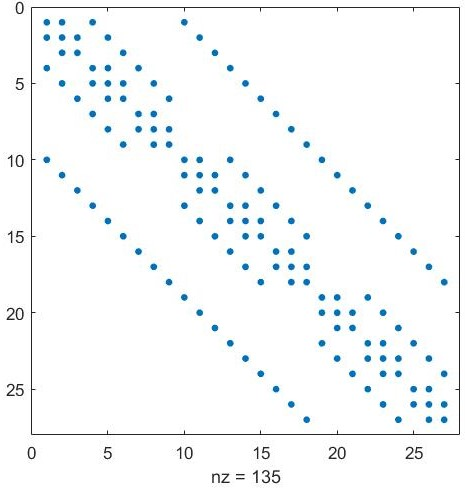
\includegraphics[width=\textwidth]{figures/sparse_8.jpg}
  \end{minipage} %
  \begin{minipage}[b]{0.49\textwidth}
    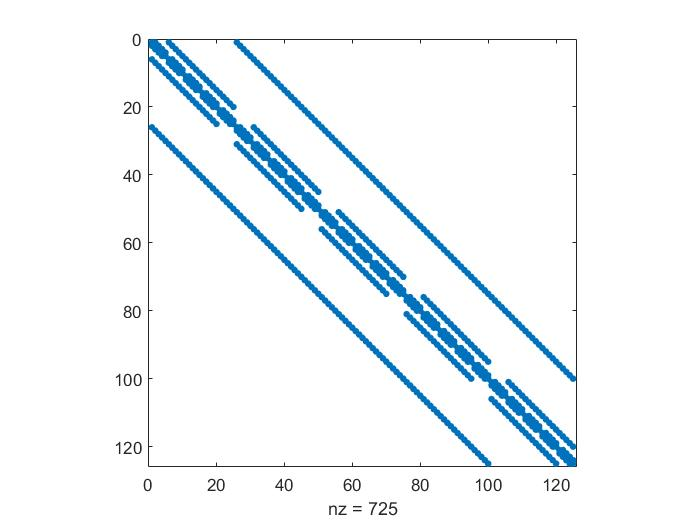
\includegraphics[width=\textwidth]{figures/sparse_64.jpg}
  \end{minipage}
  \caption[SINATRA Sparse Stencil Matrix]{SINATRA Sparse Stencil Matrix\textmd{, shown through the MATLAB\textsuperscript{\textregistered} spy command (left) 8 Cells in the mesh (right) 64 cells in the mesh.}}
  \label{fig:sparse}
\end{figure}


\Needspace{5\baselineskip}
\begin{equation}
    \label{eqn:to1D}
    Index = i \times s^2 + j \times s + k
\end{equation}
\(Index\) = The index of the 1D array \\
\(i \: \text{,} \: j \: \text{and} \: k\) = The indices of the 3D array \\
\(s\) = The size of one dimension of the 3D array \par

\Needspace{8\baselineskip}
\begin{align}\label{eqn:to3D}
    i =& \frac{Index}{s^2} \nonumber \\
    j =& \Big(\frac{Index}{s}\Big) \: \% \: s \\
    k =& Index \: \% \: s \nonumber
\end{align}
Note: Values rounded down to closest whole number for use as indices \newline
\(\%\) = The modulus operator which gives the remainder of division \par






\indent At this stage, the simulation assumes equal cell sizes and refinement across the whole domain. However, the charge density summation is calculated cell by cell, and the electric field is distributed cell by cell. These allow future iterations to have unequal cell sizes. \par


\subsection{Gauss-Seidel}
\label{sec:gauss}

The Gauss-Seidel iterative method was chosen to be the linear algebra solver for SINATRA. It was chosen for its simplicity, universality, and robustness. It has one improvement over the simplest iterative method, Jacobi, in that it uses the information as it calculates it. It solves a version of the Equation \ref{eqn:linearset}.


\Needspace{8\baselineskip}
\begin{equation}
    \label{eqn:linearset}
    A\cdot x = b
\end{equation}
In terms of SINATRA, \\
\(A\) = Stencil - Matrix of coefficients\\
\(x\) = Electric Potential - The vector to be solved \\
\(b\) = Charge Density - The calculated vector \par


The Charge Density (\(b\)), as defined in Equation \ref{eqn:density}, includes the electron density. In SINATRA the electrons are approximated with a fluid assumption as shown in the Boltzmann relationship (\ref{eqn:e_density}). This thesis will not go into a derivation of the Gauss-Seidel method, but the equation to update the electric potential at each time-step is given by Equation \ref{eqn:gauss_seidel} \footnote{A derivation of the Gauss-Seidel method can be found in Reference \cite{Gauss_eqn}}.

\begin{equation}
    \label{eqn:gauss_seidel}
    x_i^{k+1} = \Big( b_i - \sum_{j=1}^{i-1} A_{i j} x_j^{k+1} - \sum_{j=i+1}^n A_{i j} x_j^{k} \Big) / a_{ii}
\end{equation}



\indent  It was discussed previously how to distribute the ion's charge, but not how to combine the ion charge and the electron charge. Therefore, by discretizing Poisson's Equation (\ref{eqn:poisson}), combining it with Equations \ref{eqn:density} and \ref{eqn:e_density} for the charge density, and putting it in matrix form (\ref{eqn:stencil}) we get Equation \ref{eqn:mixed}. 

\Needspace{10\baselineskip}
\begin{equation}
    \label{eqn:mixed}
    A \cdot \phi = - \frac{e}{\epsilon_0} \Big[n_i - n_o \exp\Big(\frac{\phi - \phi_0}{k \: T_e}\Big)\Big]
\end{equation}
\(A\) = The sparse stencil \\
\(e\) = Charge on an electron \\
\(\epsilon_0\) = Permittivity of free space \\
\(n\) = Number density \\
\(\phi\) = Electric Potential \\
\(\phi_0\) = Initial Electric Potential \\
\(k\) = Boltzmann Constant \\
\(T_e\) = Temperature of the Electrons \par

\indent This shows that the \(b\) in Equation \ref{eqn:linearset} is the right hand side of the set of linear equations for the Gauss-Seidel solver. Importantly, note that both sides depend on the electric potential. It means that the right hand side must be recalculated at every time-step. \par
